The interface of our System is thought to be used via mobile app, because all the functionality make sense only in a \textit{movable} context (meaning, such that the user can do them anywhere they have an internet connection).

We will now list some of the user interfaces thought for \textit{Travlendar+}":

% login %
\begin{figure}[h]
	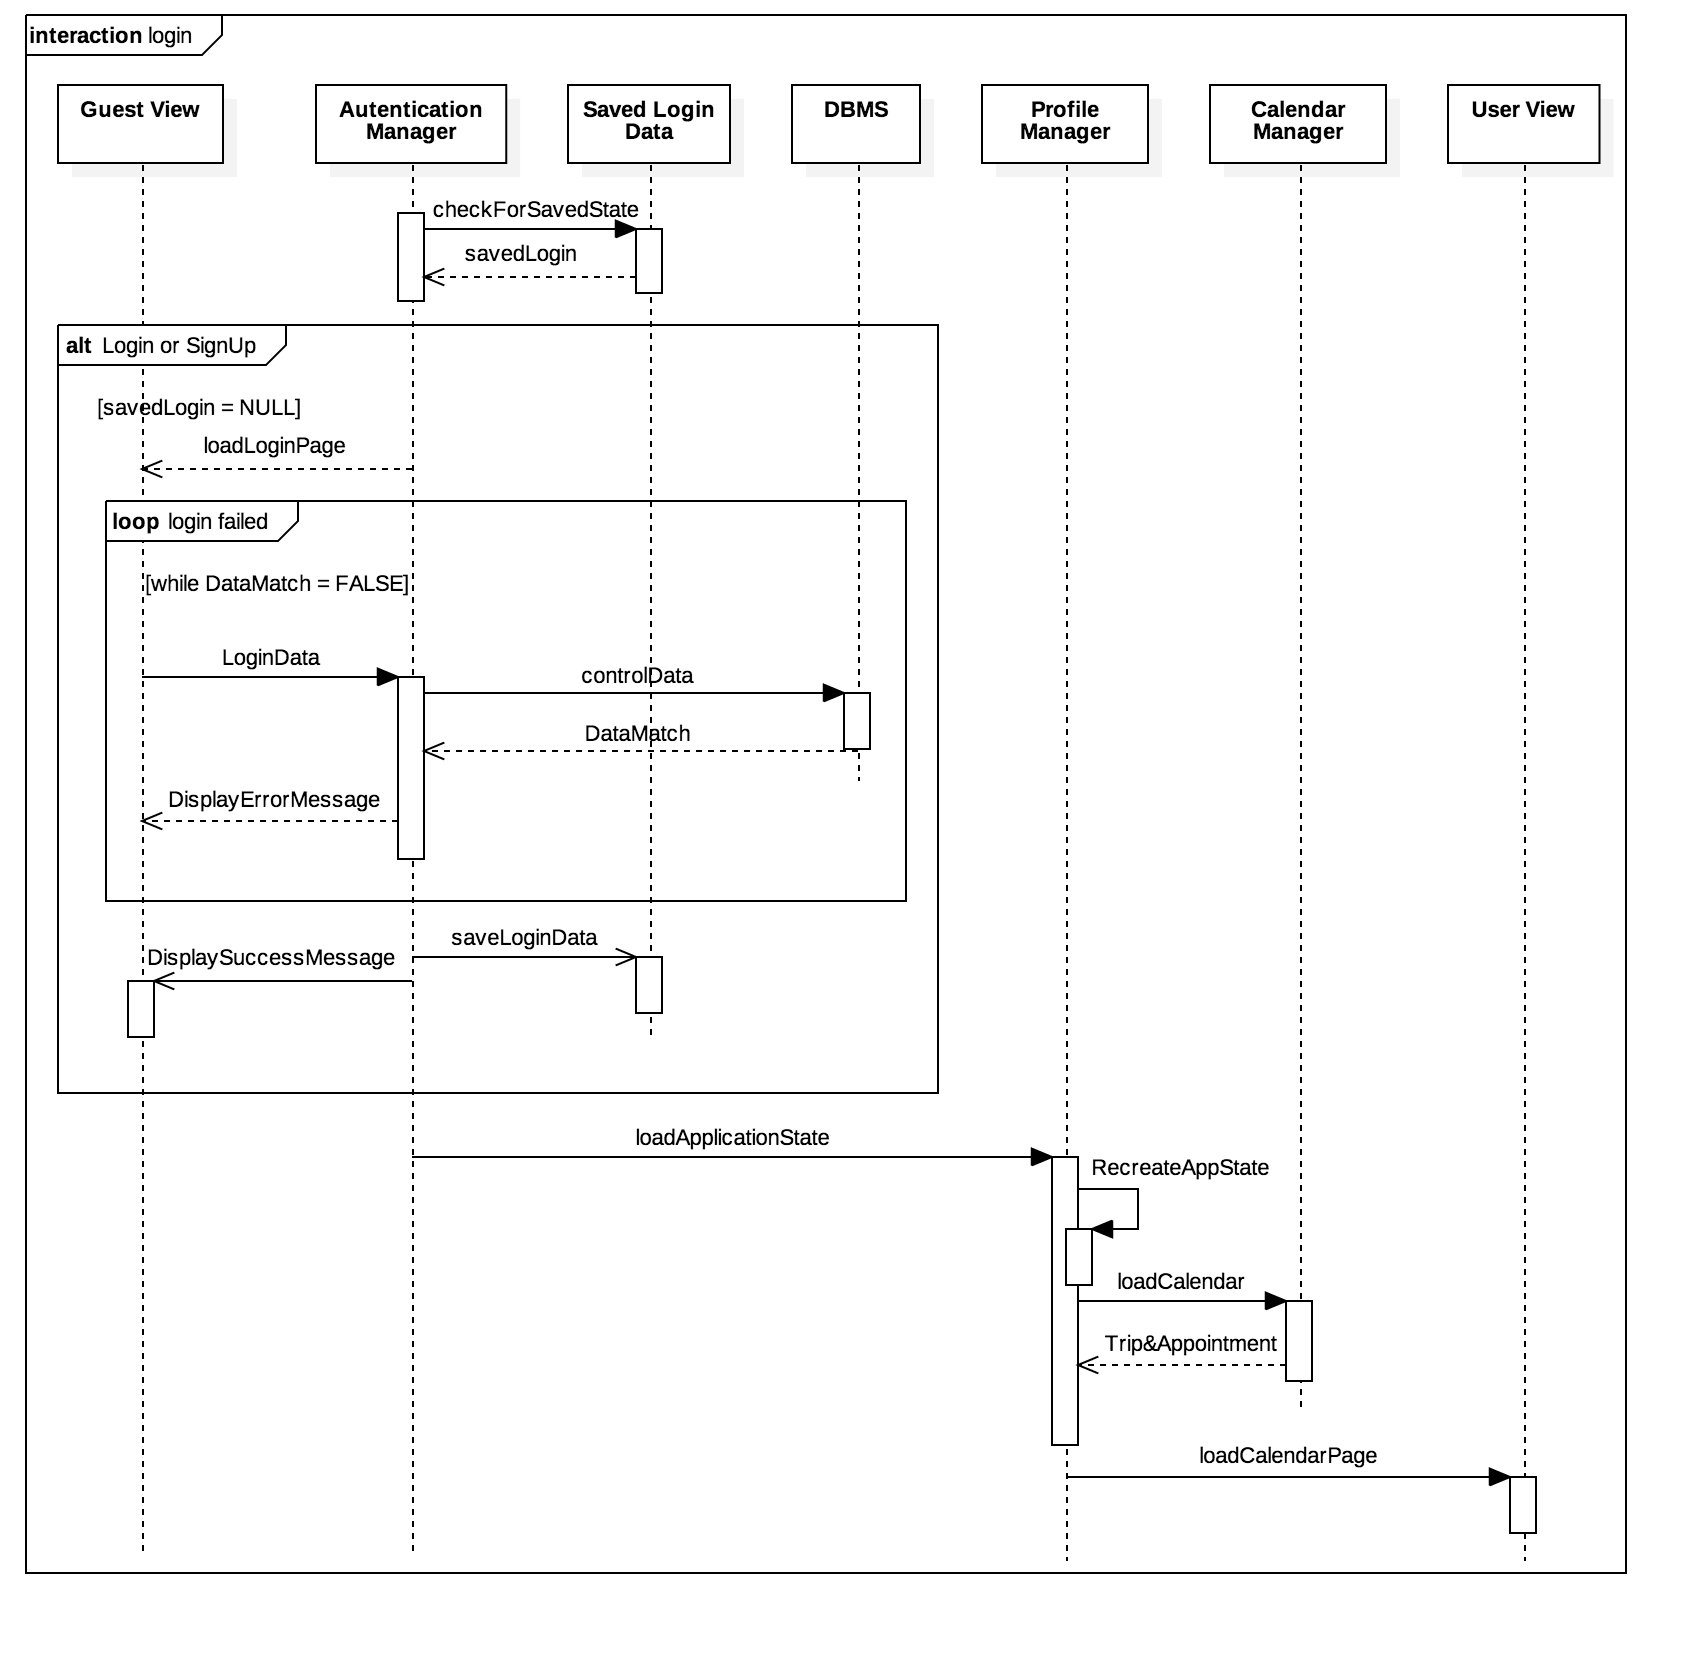
\includegraphics[width=5cm, height=9cm]{mockup/login}
	\centering
	\caption{Login Page.}
	\label{fig:login}
\end{figure}
As mentioned before, a \textit{Guest} or a \textit{non logged User} will encounter page showed in figure \ref{fig:login}, and he will never enter into the app until he completes the Login procedure (see section \ref{register_para}).
% home page %

\begin{figure}[H]
	\begin{subfigure}{0.5\textwidth}
		
\includegraphics[width=5cm, height=9cm]{mockup/homepageMonth} 
		\centering
		\caption{Home Page in Monthly view.}
		\label{fig:homePage_Month}
	\end{subfigure}
	\begin{subfigure}{0.5\textwidth}
		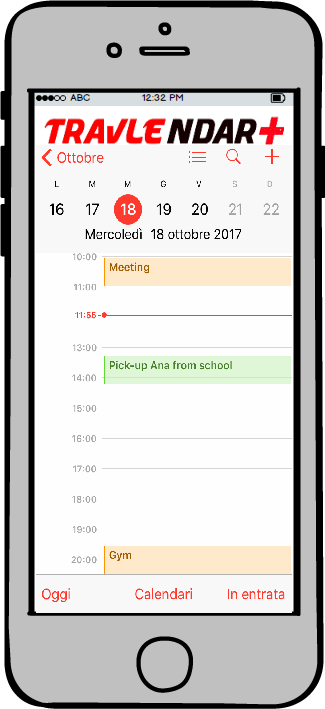
\includegraphics[width=5cm, height=9cm]{mockup/homepageDaily} 
		\centering
		\caption{Home Page in Daily view.}
		\label{fig:homePage_Day}
	\end{subfigure}
\end{figure}

\vfill